\chapter{Introdução}
\label{chap:intro}

Mais do que nunca estamos sobrecarregados com a quantidade de dados que criamos a cada dia. Quando comparamos quanto de informação vem sendo gerada nos ultimos anos, percebemos que está aumentando significamente. Além dessa evolução quantitativa, hoje temos os mais diversos tipos de informação, por exemplo: documentos, tuítes, fotos, vídeos, \textit{GIFs}, \textit{check-ins} entre vários outros.

Esse fenômeno vem sido chamado de \textit{Big Data} e representa uma crescente área de estudo atualmente. Como consequência, pesquisadores estão analisando e aprendendo com essas informações geradas, entretanto o crescimento contínuo da quantidade de dados dificulta as análises. Portanto pessoas estão investindo em novas técnicas e ferramentas para romper desafios como mineração de dados, {\em data cleaning}, visualização de dados, classificação de dados, exploração de dados e muito mais.

Um tipo comum de dados é o que chamamos de dado espacial, o qual a informação possui atributos geográficos como latitude e longitudade (por exemplo: tuítes, avaliação de restaurantes, {\em check-ins} em estabelecimentos). Dados espaciais podem ser muito significativo, por exemplo, um {\em check-in} no aeroporto por sua irmã na manhã do seu aniversário, provavelmente significa que você terá uma surpresa.

Cada registro em dados espaciais representa uma atividade numa precisa localização geográfica, em outras palavras, a análise desse tipo de dado permite realizar descobertas baseadas em fatos. Analistas estão frequetemente interessados em observar padrões espaciais e tendências para melhorar seus processos de tomada de decisão. Análise de dados espaciais tem várias aplicações como gerenciamento de cidade inteligentes, gerenciamento de disastres e transporte autônomo \cite{RoddickEHPS04,Telang:2012}.

\section{Problema}

A análise de dados espaciais geralmente é realizada num contexto exploratório: o analista não tem uma consulta precisa em mente e ele explora os dados em passos iterativos a fim de encontrar resultados potencialmente interessantes. Tradicionalmente, um cenário de análise exploratória é descrito na seguinte maneira: o analista visualiza um subconjunto de dados usando uma consulta em ambiente de visualização (por exemplo: Tableau\footnote{\it http://www.tableau.com},
Exhibit\footnote{\it http://www.simile-widgets.org/exhibit/},
Spotfire\footnote{\it http://spotfire.tibco.com}); o resultado será ilustrado em um mapa geográfico; então o analista investiga diferentes partes do conjuto de dados movendo ou focando o mapa afim de encontrar padrões ou tendências de interesse. O analista pode iterar por esse processo várias vezes realizando consultas diferentes e focando em diferentes aspectos.

Contudo, a vasto tamanho do conjunto de dados espacias faz com que o analista se sinta perdido durante a exploração. É possível ter milhares de pontos geográficos em cada bairro de uma cidade, por exemplo. Analistas precisam ter acesso apenas a algumas opções (chamadas de ``highlights'') que ajam como uma direção e assim permitir que ele foque no que lhe interessa na análise. No cenário perfeito, essas opções não são aleatoriamente escolhidas e representam o que o analista se mostrou interessado em iterações passadas.

Neste trabalho, formulamos uma solução para ``realçamento de dados usando feedback coletado ao longo do tempo''. Em outras palavras, buscamos realçar alguns pontos geográficos baseado nos interesses do analista afim de guiá-lo na direção ao que ele deve se concentrar nas iterações seguintes do processo de análise.

\subsection{Case Study}

Now, we will present a case study in order to show the functionality of our approach in practice.

\begin{figure}[t]
	\centering
	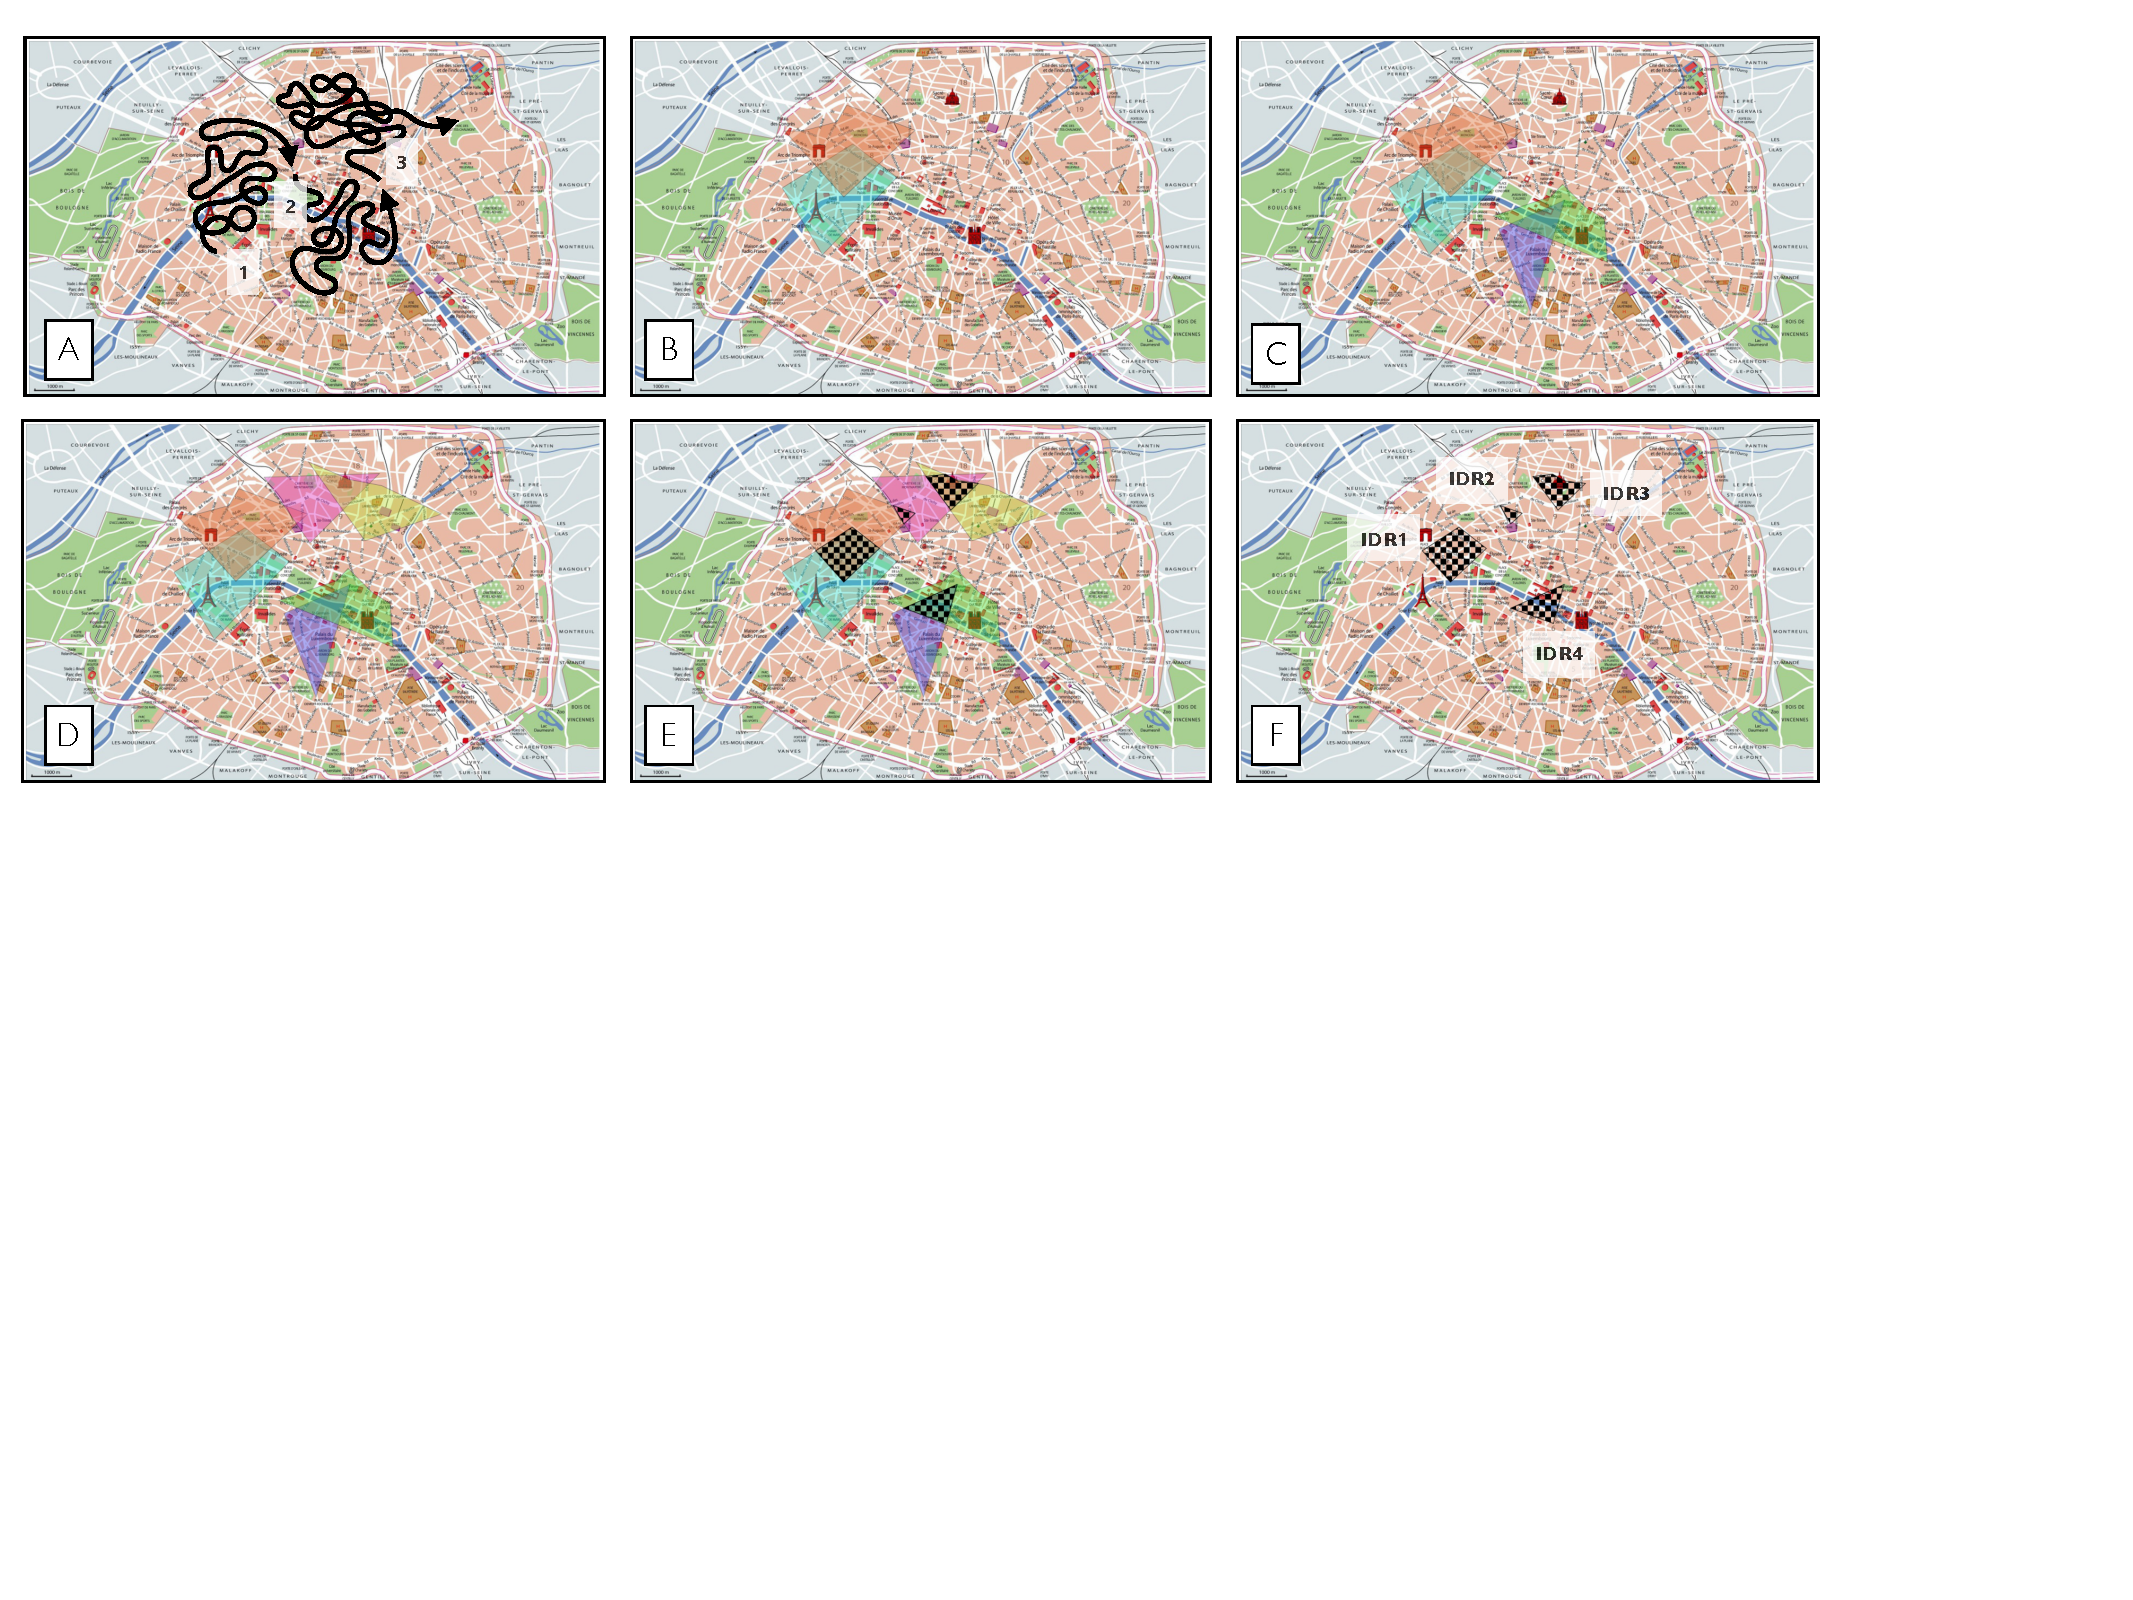
\includegraphics[width=\textwidth]{imagens/regions}
	\caption{The process of exploring Paris home-stays.}
	\label{fig:regions}
\end{figure}

{\bf Example.} {\em Lucas is planning to spend few days in Paris, France. His appreciation of French culture makes him interested in new experiences in the city. He decides to rent a home-stay from Airbnb website\footnote{\it http://www.airbnb.com}. He likes to discover the city, hence he is open to any type of lodging in any region with an interest to stay in the city center. The website returns $4000$ different locations. As he has no other preferences, an exhaustive investigation needs scanning each location independently which is nearly infeasible. While he is scanning few first options, he shows interest in the region of ``Champ de Mars'' (near Eiffel Tower), but he forgets or doesn't feel necessary to click a point there. By collecting feedback on his mouse moves over the home-stays in Paris, our system can quickly detect his interest in the region and short-list a small subset of locations (i.e., highlights) accordingly to be recommended to Lucas.}

We follow the above example to describe how implicit feedback is collected in action. Figure \ref{fig:regions} shows Lucas' steps to explore home-stays in Paris. Figure \ref{fig:regions}.A shows his mouse movements in different time stages. In this example, we consider $g = 3$ and capture Lucas' feedback in three different time segments (progressing from Figures \ref{fig:regions}.B to \ref{fig:regions}.D). It shows that Lucas started his search around Eiffel Tower and Arc de Triomphe (Figure \ref{fig:regions}.B) and gradually showed interest in south (Figure \ref{fig:regions}.C) and north (Figure \ref{fig:regions}.D) as well. All intersections between those regions are discovered (hatching regions in Figure \ref{fig:regions}.E) which will constitute the set of {\em Interesting Dense Regions} (Figure \ref{fig:regions}.F), i.e., IDR1 to IDR4.

What if Lucas wanted to come back to Paris, France next year? He will have to repeat the same exploratory analyse, unless he remember the exact location of home-stays he showed interest last year. Using our system, he won't need to remember, because his preferences were collected and can be used to highlight a subset of similar home-stays.

In the context of exploratory analysis, the analyst may change his preferences between session (e.g., in the winter, Lucas may want to be close to the Eiffel Tower, but in the summer, he may not). In order to tackle this challenge we also apply a temporal analyse to identify patterns in how the analyst preferences change between sessions which allow our highlighting method to be more precise and consistent to the analyst interest.

\section{Objectives}

In this section, we define the general and specific objectives of our work.

\subsection{General Objectives}

\begin{itemize}
	\item Introduce a time-aware guidance approach for spatial data exploration;
	\item Elaborate how temporal analyses can be effectively applied in data exploration;
\end{itemize}

\subsection{Specific Objectives}

\begin{itemize}
	\item Describe our data model used for temporal analyses;
	\item Describe our concept of {\em Interesting Dense Regions} used for collecting feedback;
	\item Present the results of our guidance approach.
\end{itemize}

\section{Organization}

The next chapters is as follow: in the Chapter \ref{chap:background} we discuss the background of this work. Chapter \ref{chap:model} defines the data model. Chapter \ref{chap:collecting} presents how the feedback is collected during exploration. Chapter \ref{chap:applying} presents how temporal analysis is applied. Chapter \ref{chap:guiding} presents how highlight interesting points in order to guide the user using collected feedback and results from temporal analysis. Chapter \ref{chap:experiments} shows experiments and its results. Chapter \ref{chap:conclusion} presents some conclusions and future directions.
